%-------------------------------------------------------------------------------
% port_mapping
%-------------------------------------------------------------------------------
%
% \file        port_mapping.tex
% \library     Documents
% \author      Chris Ahlstrom
% \date        2020-12-29
% \update      2023-06-26
% \version     $Revision$
% \license     $XPC_GPL_LICENSE$
%
%     Provides a discussion of the MIDI GUI port_mapping that Seq66
%     supports.
%
%-------------------------------------------------------------------------------

\section{Port Mapping}
\label{sec:port_mapping}

   \textsl{Seq66}, like \textsl{Seq24}, bases its I/O port scheme on buss/port
   \textsl{numbers}.
   This numbering scheme applies whether
   \textsl{ALSA}, \textsl{JACK}, or \textsl{Windows Multimedia}
   are used as the MIDI engine, and whether \textsl{Seq66} is running with
   "automatic" ports or "manual" (virtual, software-created) ports.
   These buss numbers range from 0 on upward
   based on the number of I/O MIDI ports active in the system.
   In "automatic" (non-virtual, non-manual) mode
   these ports represent the hardware MIDI ports and application MIDI ports.
   In "manual" mode, these ports represent virtual MIDI ports that the user
   can connect manually (on Linux).

   \textbf{Note}:
   \textsl{Port-mapping is now automatic; default MIDI I/O port-maps are
   created at first start, and are always active if virtual ports are not in
   use.  Once created, one can edit the 'rc' file to rearrange the mapping as
   desired.
   In addition, issues with new or unavailable ports are
   noted in warning dialogs.
   (The startup warnings can be suppressed;
   see \sectionref{paragraph:menu_edit_preferences_display}.)
   The user can click the \textbf{Remap and restart} button,
   fix the loaded pattern to use existing ports,
   or exit, determine the existing ports using
   \texttt{aplaymidi}, \texttt{arecordmidi}, or \texttt{jack\_lsp},
   and edit the maps directly in the 'rc' file.}

   The output bus or port for a given pattern can be determined by
   looking at the grid slots or by dumping a summary of the song to
   a text file.
   See \sectionref{subsubsec:menu_help_song_summary_file}.

   A pattern/loop/sequence is assigned to output to a given port via
   a buss number saved \textsl{in the pattern}, in the tune.
   When a tune is loaded,
   each pattern outputs to the port number specified in the pattern.
   A problem is that MIDI device setups can change, with devices being
   reordered, removed, or added to the MIDI devices available on the system.
   Or if the song is opened on someone else's computer.
   We do not want to store port names in the MIDI file.
   They can be too long, but, more importantly,
   they will differ between the systems of each user.
   They can even differ when switching from ALSA to JACK, or even versions
   of these MIDI engines.
   Better to let the user determine the port-mapping.
   Mapping allows the buss number stored with a pattern to be
   remapped to another buss number based on the "nick-name"
   (or JACK alias) of the port.
   It uses a simple lookup to map names to numbers.

   The "nick-name" is a shortened version of the MIDI device name assigned
   by the system.
   For example, the long name of a MIDI port might be
   \texttt{[5] 44:0 E-MU XMidi1X1 Tab MIDI 1}.
   The nick-name is \texttt{E-MU XMidi1X1 Tab MIDI 1}.
   In order find the correct port number, the long name is checked to see if it
   \textsl{contains} the nick-name, and, if so, the corresponding port number is
   returned.  The user can edit the 'rc' file to shorten the nick-name, if
   desired; a nick-name \texttt{E-MU XMidi1X1} would work.

   In addition, under recent versions of \textsl{JACK},
   there is a facility to get the "alias" of USB MIDI ports,
   even if the \textsl{a2jmidid} process is not running.
   This allows the user to see that the port name
   \texttt{system:midi\_capture\_5} is actually a "nanoKEY2" device.

   So, with port-mapping enabled, one can set up the tune to record and play
   MIDI using the mapped ports, and later move to another computer, modify the
   port-maps int the 'rc' file to match, and record and play without issue.

   The easiest way to start port-mapping (which is now automatic) is to go to
   \textbf{Edit / Preferences / MIDI Clock}.
   Here, we see the long MIDI port names made up by the system, along
   with the \textsl{JACK} aliases that can be retrieved, and which make it easy
   to see which devices are in play.

\begin{figure}[H]
   \centering 
   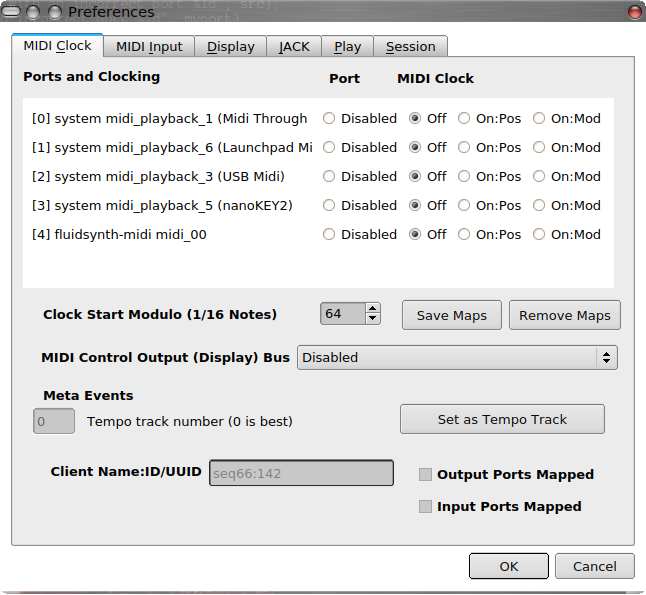
\includegraphics[scale=0.75]{main-menu/edit/preferences/midi_clock_pre_portmap.png}
   \caption{Clocks List Before Port Mapping}
   \label{fig:clocks_list_before_port_mapping}
\end{figure}

   Click on the \textbf{Make Maps} button.
   This creates the initial I/O maps internally.
   Then either restart \textsl{Seq66} or go to the \textbf{Restart Seq66}
   button; this will save the new version of the 'rc' file..
   Back in \textbf{Edit / Preferences / MIDI Clock},
   one sees that the remapped names are in use.

\begin{figure}[H]
   \centering 
   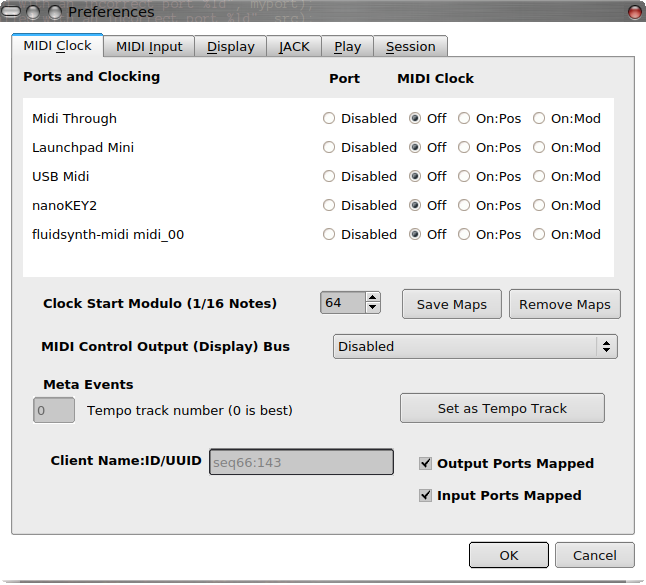
\includegraphics[scale=0.75]{main-menu/edit/preferences/midi_clock_post_portmap.png}
   \caption{Clocks List After Port Mapping}
   \label{fig:clocks_list_after_port_mapping}
\end{figure}

   At startup, \textsl{Seq66} matches the port-map to the ports that exist on
   the system.  If there is no matching system port for a mapped port, then
   that mapped port will show up as disabled in the port lists,
   and a warning should appear.
   To remove the port mappings, click the \textbf{Clear Maps} button.
   To reconstruct the current setup, click on the \textbf{Make Maps} button to
   get the new mapping.
   As with the normal port listings, the port-mappings are saved and
   managed in the \textsl{Seq66} 'rc' file.
   One can also edit that file in a text editor to
   rearrange the mapped ports.

   Note that one can also deactivate port-mapping.

\subsection{Output Port Mapping}
\label{subsec:output_port_mapping}

   Assume that the system has the following set of ports.  These busses are
   stored in the 'rc' file when \textsl{Seq66} exits.  Note the \textsl{JACK}
   aliases shown at the right as comments.

   \begin{verbatim}
      [midi-clock]
       5      # number of MIDI clocks (output busses)
       0  0   "[0] 0:0 seq66:system midi_playback_1"    # 'Midi Through'
       1  0   "[1] 0:1 seq66:system midi_playback_6"    # 'Launchpad Mini'
       2  0   "[2] 0:2 seq66:system midi_playback_3"    # 'USB Midi'
       3  0   "[3] 0:3 seq66:system midi_playback_5"    # 'nanoKEY2'
       4  0   "[4] 1:4 seq66:fluidsynth-midi midi_00"
   \end{verbatim}

   If some items are unplugged, then this list will change, so we save it while
   still running \textsl{Seq66}:
   click the
   \textbf{Make Maps} button in the
   \textbf{Edit / Preferences/ MIDI Clock} dialog. 
   The result is are new sections in the 'rc' file (one for clocks, one for
   inputs).  Here is the clock map:

   \begin{verbatim}
      [midi-clock-map]
       1      # map is active
       0  0   "Midi Through"
       1  0   "Launchpad Mini"
       2  0   "USB Midi"
       3  0   "nanoKEY2"
       4  0   "fluidsynth-midi midi_00"
   \end{verbatim}
   
   It is simpler, showing the nick-names (or aliases) of the ports.
   These index numbers can be used as buss numbers: they can be stored
   in a pattern, and used to direct output to a specific device.

   If a pattern has stored a missing item as its output
   buss number, this number will not be found in the system list, so that the
   pattern will need to be remapped to an existing port.

   Note that the mapping can be disabled by setting the first value to 0.  In
   that case, \textsl{Seq66} uses buss numbers in the normal way.
   In the user interface dropdowns for output buss, if a map is active, it is
   put into the dropdown; any missing items are noted and are shown as
   disabled.

   If the map is not active, then only the actual system output ports are
   shown in the user interface.

\subsection{Input Port Mapping}
\label{subsec:input_port_mapping}

   The input ports are handling somewhat similarly.  Here's another
   initial system input setup:

   \begin{verbatim}
       4      # number of input MIDI busses
       0  1   "[0] 0:0 seq66:system midi_capture_1"     # 'Midi Through'
       1  1   "[1] 0:1 seq66:system midi_capture_6"     # 'Launchpad Mini'
       2  1   "[2] 0:2 seq66:system midi_capture_3"     # 'USB Midi'
       3  1   "[3] 0:3 seq66:system midi_capture_5"     # 'nanoKEY2'
   \end{verbatim}

   Note that the "system:announce" buss is always disabled, as \textsl{Seq66}
   does not use it (yet).  Here is the stored input port-map:

   \begin{verbatim}
      [midi-input-map]
       1      # map is active
       0  1   "Midi Through"
       1  1   "Launchpad Mini"
       2  1   "USB Midi"
       3  1   "nanoKEY2"
   \end{verbatim}

   Other than being input devices, this input map works like the output
   (clocks) map.
   In the user interface dropdowns for input buss, if a map is active, it is
   put into the dropdown; any missing items are noted and are shown as
   disabled.
   If the map is not active, then only the actual system input ports are shown.

\subsection{Port Mapping Example}
\label{subsec:input_port_mapping_example}

   This example shows that MIDI control and MIDI status displays work with
   port mapping.  First, we run \textsl{Seq66}, save the ports for
   remapping, and exit the application.  Looking in the 'rc' file, we tweak
   the maps:

   \begin{verbatim}
      [midi-input-map]
      1       # map is active
      0  0    "announce"
      1  0    "Midi Through Port-0"
      2  0    "Launchpad Mini MIDI 1"
      3  0    "nanoKEY2 MIDI 1"
      4  0    "Q25 MIDI 1"
      5  0    "E-MU XMidi1X1 Tab MIDI 1"
   \end{verbatim}

   And:

   \begin{verbatim}
      [midi-clock-map]
      1       # map is active
      0  0    "Midi Through Port-0"
      1  0    "Launchpad Mini MIDI 1"
      2  0    "nanoKEY2 MIDI 1"
      3  0    "Q25 MIDI 1"
      4  0    "E-MU XMidi1X1 Tab MIDI 1"
   \end{verbatim}

   These two maps reflect the configuration at the time they were saved.
   They reflect the output of \texttt{arecordmidi -{}-list} and
   \texttt{aplaymidi -{}-list}.
   After unplugging and replugging some devices, we see that the
   \textsl{Launchpad Mini} has moved:

   \begin{verbatim}
      6   # number of input MIDI busses
      3 0    "[3] 36:0 Launchpad Mini MIDI 1"

      5   # number of MIDI clocks (output busses)
      2 0    "[2] 36:0 Launchpad Mini MIDI 1"
   \end{verbatim}

   On input, it has moved from buss 2 to buss 3.
   On output it has moved from buss 1 to buss 2.
   This can be verified by running \textsl{Seq66}, immediately exiting,
   and checking the \texttt{qseq66.rc} file.
   We edit that file to add:

   \begin{verbatim}
      [midi-control-file]
      "qseq66-lp-mini-alt.ctrl"
   \end{verbatim}

   With the I/O maps shown above active in the 'rc' file,
   we can go to the 'ctrl' file (\texttt{qseq66-lp-mini-alt.ctrl}, available in
   the \texttt{data/linux} install/source directory)
   and set the following:

   \begin{verbatim}
      [midi-control-settings]
      control-buss = 2              # maps to system input buss 3
      midi-enabled = true

      [midi-control-out-settings]
      output-buss = 1               # maps to system output buss 2
      midi-enabled = true
   \end{verbatim}

   With this setup, the lights on the Mini light-up at start-up, and the
   buttons control the pattern, mute-groups, and automation features set up in
   the above-mentioned 'ctrl' file.
   The buss number will be replaced with the name of the
   device, e.g. \texttt{output-buss = "Launchpad Mini"}, if port-mapping
   is active.

   Perhaps tricky, but once one has set up a whole suite of I/O device maps,
   one can reliably use these mapped port numbers to look up the actual
   system port numbers.  For example, with the above setup, \textsl{Seq66} can
   be assured that output buss 1 will always go to the
   \textsl{Launchpad Mini}.

%-------------------------------------------------------------------------------
% vim: ts=3 sw=3 et ft=tex
%-------------------------------------------------------------------------------
